\texttt{Consegna:}
\begin{enumerate}
    \item \textbf{Lighting}: permettere lo spostamento interattivo della luce posizionale/direzionale in scena
    \item \textbf{Shading}: realizzare la modalità shading Phong realizzando gli shaders \texttt{v\_phong.glsl} e \texttt{f\_phong.glsl} 
    \item \textbf{Texture mapping 2D} del toro con immagine letta da file utilizzando gli shaders \texttt{v\_texture.glsl} e \texttt{f\_texture.glsl}.
    \item \textbf{Texture mapping 2D + Shading} Realizzare gli shaders \texttt{v\_texture\_phong.glsl} e \texttt{f\_texture\_phong.glsl} per combinare l'effetto shading Phong con la texture image sulla mesh toro
    \item \textbf{Procedural mapping} basato su un procedimento algoritmico a piacere sul toro
    \item \textbf{Wave Motion} creare l'animazione dell'oggetto \textit{GridPlane} modificando la posizione dei vertici in un vertex shader \texttt{v\_wave.glsl}. Utilizzando la variabile elapsed time \textit{t}, passata da applicazione al vertex shader, per riprodurre il moto ondoso ottenuto con la sola modifica della coordinata y.
    \item \textbf{Toon Shading}: realizzare gli shaders \texttt{v\_toon.glsl} e \texttt{f\_toon.glsl} per la resa non fotorealistica nota comunemente come Toon Shading
    
\end{enumerate}
\texttt{Svolgimento:}
Nuovamente è stato trovato un problema di compatibilità, in particolare la versione utilizzata negli shader. Per farli funzionare nella mia macchina, ho deciso di settarli a 320 es, ma questo ha provocato un ulteriore problema, la mancanza di precisione. Quest'ultimo punto è stato risolto inserendo la linea di codice \textit{\#precision mediump float}. La scelta del medium è per avere ulteriori problemi di compatibilità, in caso dovessi cambiare architettura hardware.\\ Nuovamente, sono stati inseriti dei path assoluti, precisamente \textbf{MeshDir}, \textbf{TextureDir} e \textbf{ShaderDir}, che devono essere modificati per testare il programma.
\begin{enumerate}
    \item \textbf{Lighting}: Selezionando l'oggetto luce, e selezionando una \textit{OperationMode} diversa dalla \textbf{Navigazione}, si arriverà ad invocare la funzione \textit{modifyModelMatrix}. Il suo contenuto è lo stesso della esercitazione3, a differenza che in questo caso non abbiamo una matrice di float, ma un mat4, ma il ragionamento dietro è lo stesso. All'interno della funzione vi è stata aggiunta la parte per la gestione anche della luce vera e propria, modificandone la posizione grazie all'attributo \texttt{light.position}.\\ Ma ciò non è sufficiente a notare, durante l'esecuzione, un cambiamento. Questo perché nella funzione \textit{display} non venivano modificati, di volta in volta, il contenuto di \textbf{light\_uniforms[SHADER]}, ma erano stati assegnati solo durante l'inizializzazione degli shaders. Aggiungendo quelle righe a tutti gli shader, è stato possibile completare la consegna.
    \item \textbf{Shading}: l'algoritmo di Phong è stato implementato negli shader\texttt{v\_phong.glsl} e \texttt{f\_phong.glsl}, e per capire come programmare uno shader sono stati utilizzati gli shaders di Blinn e Gouraud come esempi.
    \\
           {\centering
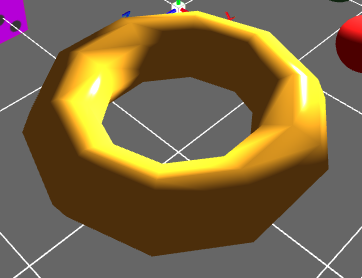
\includegraphics[width=0.6\textwidth]{toroPhong.png}} 
    \item \textbf{Texture mapping 2D}: dopo aver modificato la funzione \textit{init\_torus} con gli appositi parametri, mi sono reso conto che ciò non era sufficiente, in quanto la texture non veniva applicata correttamente. Per questo è stato aggiunto alla funzione \textit{computeTorusVertex} l'inizializzazione delle coordinate Texture.
    \\
           {\centering
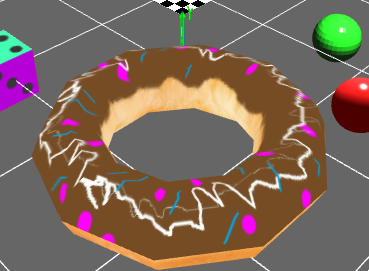
\includegraphics[width=0.6\textwidth]{toroTexture.png}} 
    \item \textbf{Texture mapping 2D + Shading}: nuovamente sono stati presi come base due shaders per creare quello richiesto, \textbf{Texture\_Only}, dato già nella esercitazione, e Phong, creato per un punto precedente.  \\
           {\centering
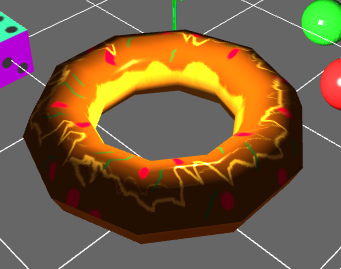
\includegraphics[width=0.6\textwidth]{toroTexturePhong.png}} 
    \item \textbf{Procedural mapping} Utilizzando la funzione \textit{generate\_texture}, che era già presente perla generazione della texture scacchiera su un piano,
    sono state create due funzioni, \textit{generateShadesOfGray} e \textit{generateRainbowMap}. La prima mi è servita per capire come lavorare sul toro, e come la texture veniva mappata sul toro. La seconda, esteticamente magari più piacevole, mi ha permesso di capire come modificare i colori nella zona selezionata.\\
          {\centering
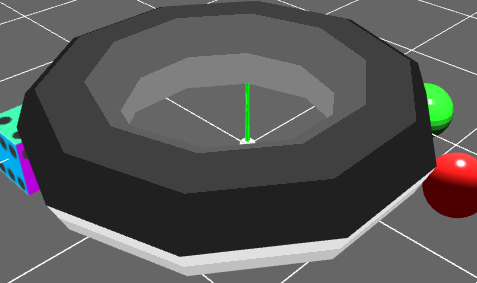
\includegraphics[width=0.6\textwidth]{toroGrey.png}}\\
{\centering
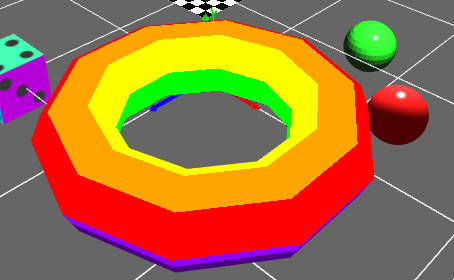
\includegraphics[width=0.6\textwidth]{toroArcobaleno.png}}
    \item \textbf{Wave Motion}: La costruzione prevede varie parti: la prima è l'inizializzazione della wave, effettuata nella funzione \textit{init\_wave}. Successivamente c'è la parte di configurazione dello shader, simile agli altri, con solo la differenza che gli viene passato anche il parametro \textit{t}, richiesto dall'esercizio e ottenuto attraverso \textit{glutGet(GLUT\_ELAPSED\_TIME)}. Per poter attivare il movimento è stata aggiunta una nuova opzione nel menù, \textbf{Move waves}, che attiverà \textit{glutIdleFunc} della mia callback, \textit{moveWaves}. Questa funzione non fa altro che richiamare costantemente lo shader sull'oggetto, con il nuovo valore di \textbf{waveTime}.\\ Lo shader è abbastanza lineare, come il vertex shader \texttt{v\_passthrough.glsl} ottiene la posizione e, applicando la formula inserita nella richiesta dell'esercitazione, calcola la nuova posizione. Sono state aggiunte anche le righe di codice necessarie al passaggio di una texture, in quanto mi sembrava troppo brutto lasciarlo bianco.\\
        {\centering
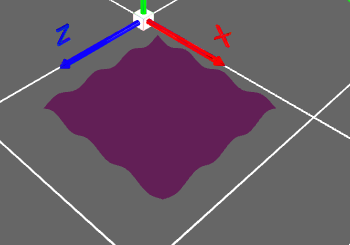
\includegraphics[width=0.6\textwidth]{wave.png}}
    \item \textbf{Toon Shading} L' idea per creare il toon shading è abbastanza semplice: si considerano intervalli fissi di luce, nel mio caso sono 4 intervalli limitati dai valori 30, 60 e 80 e ogni punto, a seconda della intensità della luce che lo colpisce, viene reso più luminoso moltiplicando il colore base per un valore costante a seconda dell'intervallo in cui cade. Il resto del codice di  \texttt{v\_toon.glsl} e \texttt{f\_toon.glsl}  è lo stesso degli altri shaders. \\
    {\centering
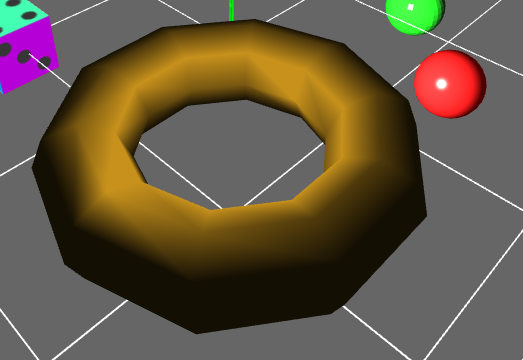
\includegraphics[width=0.6\textwidth]{toroToon.png}}

\end{enumerate}
% PANDA ciao poci ciao